% This template is adapted from the CS224N Spring 2024 Project Milestone Template 
% https://web.stanford.edu/class/archive/cs/cs224n/cs224n.1246/project/project-milestone-instructions-spr2024.pdf

\documentclass{article}

\usepackage[final]{neurips_2019}
\setcitestyle{numbers}  % Force numerical citations

\usepackage[utf8]{inputenc}
\usepackage[T1]{fontenc}
\usepackage{hyperref}
\usepackage{url}
\usepackage{booktabs}
\usepackage{amsfonts}
\usepackage{amsmath}
\usepackage{nicefrac}
\usepackage{microtype}
\usepackage{graphicx}
\usepackage{xcolor}
\usepackage{lipsum}
\usepackage{booktabs}
\usepackage{makecell}

\newcommand{\note}[1]{\textcolor{blue}{{#1}}}

\title{
  Multitask Training with BERT \\
  \vspace{1em}
  \small{\normalfont Stanford CS224N Default Project} 
}

\author{
  Ruining Luo \\
  School of Computing and Data Science \\
  The University of Hong Kong\\
  \texttt{ning.l.rn@connect.hku.hk} \\
}
  % Examples of more authors
%   \And
%   Name \\
%   Department of Computer Science \\
%   Stanford University \\
%   \texttt{name@stanford.edu} \\
%   \And
%   Name \\
%   Department of Computer Science \\
%   Stanford University \\
%   \texttt{name@stanford.edu}

\begin{document}

\maketitle

\begin{abstract}
  %Your abstract should motivate the problem, describe your goals, and highlight your main findings. Given that your project is still in progress, it is okay if your findings are what you are still working on.
  This project consists of completing an implementation of the BERT model and exploring various techniques
  for improving its performance on multiple sentence-level tasks with multi-task learning,
  as conducted for the CS 224N final project. 
  The models are fine-tuned for sentiment analysis, paraphrase detection, and semantic textual similarity with three corresponding datasets,
  the Stanford Sentiment Treebank (SST) dataset, the Quora dataset, and the the SemEval STS Benchmark dataset.
  The experimental results show that techniques including paired encoding, PCGrad, and gradient clipping are helpful in increasing the overall performance of the model.\\
  \textit{This report is formatted as a simplified conference paper to document the methodology and results of an independent study on the course CS 224N.}
\end{abstract}

% {\color{red} This template does not contain the full instruction set for this assignment; please refer back to the milestone instructions PDF.}

\section{Approach}
%3This section details your approach to the problem. 
%\begin{itemize}
%    \item Please be specific when describing your main approaches. You may want to include key equations and figures (though it is fine if you want to defer creating time-consuming figures until the final report).
%    \item Describe your baselines. Depending on space constraints and how standard your baseline is, you might do this in detail or simply refer to other papers for details. Default project teams can do the latter when describing the provided baseline model.
%    \item If any part of your approach is original, make it clear. For models and techniques that are not yours, provide references.
%    \item If you are using any code that you did not write yourself, make it clear and provide a reference or link. 
%    When describing something you coded yourself, make it clear.
%\end{itemize} 
  \subsection{Main Approaches}

    \paragraph{Pretrained BERT}
      This project utilizes pretrained BERT model weights and embeddings from a local BERT model ("bert-base-uncased") \cite{devlin2019bert}, and attempts to fine-tune the model to improve its performance on the three tasks.
      The code of the BERT model is largely given and the implementation is done by filling missing code blocks. 

    \paragraph{Multitask training}
      Rather than fine-tuning on the three tasks independently, the project aims to improve the performance by training over the three tasks simultaneously.
      The total loss is the sum of losses on all three tasks as proposed by \cite{bi2022mtrec}.
      \begin{equation}
        \mathcal{L}_{total} = \mathcal{L}_{sentiment} + \mathcal{L}_{paraphrase} + \mathcal{L}_{similarity}
      \end{equation}
      We also experimented with a version of uncertainty weighted loss introduced by Kendall et al.\cite{kendall2018multi},
      where  log-variance parameters $s_{task}$ are introduced and learned to penalize more uncertain updates.
      \begin{equation}
        \mathcal{L}_{total} = \sum_{task} s_{task} \mathcal{L}_{task} + s_{task}
      \end{equation}

    \paragraph{Oversampling and undersampling}
      Since the Quora dataset is significantly larger than the other two datasets, we experimented with oversampling and undersampling to address the class imbalance\cite{mohammed2020machine}.
      In earlier experiments, the number of steps of each epoch is the size of the Quora dataset.
      At each step, examples are drawn from all three datasets, so the SST and STS datasets are iterated over multiple times.
      While the accuracy of paraphrase detection rises stably with time, the score of sentiment analysis and semantic textual similarity do not converge properly.
      This indicates that the Quora dataset dominates the training.
      Later, the number of steps of each epoch is set to the size of the smallest dataset.
      It proves that undersampling leads to better convergence and helps prevent domination by one dataset.

    \paragraph{PCGrad (Gradient Surgery)}
      To mitigate potential conflicts among tasks in multi-task training, we implemented the PCGrad algorithm proposed by Yu et al.\cite{yu2020gradient}.
      It detects if the gradients $\mathbf{g}_i, \mathbf{g}_j$ of the $i$-th, $j$-th tasks have negative dot-product,
      and projects one gradient onto the normal plane of another gradient:
      \begin{equation}
        \mathbf{g}_i = \mathbf{g}_i - \frac{\mathbf{g}_i \cdot \mathbf{g}_j}{\lVert \mathbf{g}_j \rVert^2} \cdot \mathbf{g}_j
      \end{equation}

    \paragraph{Sample weighted PCGrad}
      To address the potential statistical effect of the unbalanced sizes of datasets, we attempted to weigh the PCGrad updates with respect to the sizes of the datasets:
      \begin{equation}
        \mathbf{g}_{task_i} = \frac{\mathbf{g}_{task_i}}{\mathrm{Size}_{task}}
      \end{equation}


    \paragraph{MLP prediction heads}
      The provided code originally utilizes independent linear classifiers for each task.
      Passing embeddings into MLP layers proves to give better performance.

    \paragraph{"Paired encoding"}
      In the original code, for paraphrase detection and semantic textual similarity, two sentences are passed independently to BERT and the prediction is based on the concatenation of two embeddings.
      We modified the dataloaders to concatenate the sentence tokens with a SEP token in between, and use the result to produce a single embedding for prediction\cite{devlin2019bert}.
      This leads to a substantial increase in performance, especially for semantic textual analysis. As there seems to be no specific name for this method, it is referred to as "paired encoding" in the report.


    \paragraph{Cosine similarity and CosineEmbeddingLoss}
      Given that sentence embeddings have an intrinsic notion of cosine similarity, we also experimented with simple cosine similarity and CosineEmbeddingLoss\footnote{https://pytorch.org/docs/stable/generated/torch.nn.CosineEmbeddingLoss.html} on the SemEval dataset.

  \subsection{Baseline}
    When training the first model with undersampling, we found that the performance is similar to earlier oversampling models although it requires much less time to train.
    Therefore, all later models are trained with undersampling, with the same training time of 50 epochs.
    For consistency and convenience, we use the model with undersampling and MLP prediction heads as baseline.

\section{Experiments}
%This section is expected to contain the following.
%\begin{itemize}
%    \item \textbf{Data}: Describe the dataset(s) you are using along with references. Make sure the task associated with the dataset is clearly described.\\
%    \item \textbf{Evaluation method}: Describe the evaluation metric(s) you used, plus any other details necessary to understand your evaluation.
%    \item \textbf{Experimental details}: Please explain how you ran your experiments (e.g. model configurations, learning rate, training time, etc.).
%    \item \textbf{Results}: Report the quantitative results that you have so far. Use a table or plot to compare multiple results and compare against your baselines.
%\end{itemize}
  \subsection{Data}
    The datasets employed are default datasets provided by the project.
    For sentiment analysis, we employed the Stanford Sentiment Treebank (SST) dataset\footnote{https://nlp.stanford.edu/sentiment/treebank.html}\cite{socher2013recursive}, 
    which consists of 11,855 single sentences from movie reviews labelled with negative, somewhat negative, neutral, somewhat positive, or positive.
    For paraphrase detection, we employed the Quora dataset\footnote{https://www.quora.com/q/quoradata/First-Quora-Dataset-Release-Question-Pairs},
    which consists of 404,298 question pairs labelled whether the questions are paraphrases of one another.
    For semantic textual similarity, we employed the SemEval STS Benchmark dataset\footnote{https://aclanthology.org/S13-1004.pdf}\cite{agirre2013sem},
    which consists of 8,528 sentence pairs with similarity scores ranging from 0 (unrelated) to 5 (equivalent).

  \subsection{Evaluation Method}
    We utilize prediction accuracy for sentiment analysis and paraphrase detection,
    and Pearson correlation of the true similarity values against predicted values for semantic textual similarity.
    The metric for overall performance is the collective performance over the three tasks (as in the project description).
    \begin{equation}
    \mathrm{Score} = \frac{1}{3} \times \mathrm{Acc_{sentiment}} + \frac{1}{3} \times \mathrm{Acc_{paraphrase}} + \frac{1}{3} \times \frac{\mathrm{Corr_{similarity}} + 1}{2}
    \end{equation}

  \subsection{Experimental Details}

    \paragraph{Training and Hyperparameters} All models are trained with the following hyperparameters and undersampling for 50 epochs on a single cloud RTX4090 GPU.
      \begin{itemize}
        \item Learning rate of $1\mathrm{e}^{-5}$
        \item Batch size of 32
        \item BERT hidden size of 768
        \item MLP hidden size of 768
        \item Dropout rate of 0.1
      \end{itemize}
    
    \paragraph{Experimentation process} We first conducted multiple experiments with oversampling.
    The models have worse performance than the vanilla undersampling model\ref{fig:1}.
    The vanilla undersampling model is set as the baseline, and the training data of the oversampling models are not included in the report.\\
    Since the model still underperforms in semantic textual similarity, we experimented with cosing similarity loss and CosineEmbeddingLoss,
    which prove to have no significant impact.\\
    Then, we utilize pairwise encoding to let the attention mechanism to better capture the similarity relationship between sentences.
    It greatly increases the performance on STS Correlation and also Paragraph Detection Accuracy.\\
    Noticing the oscillation in Sentiment Analysis Accuracy\ref{fig:2}, we hyphothesized that the unbalanced dataset sizes might be an issue.
    We also hyphothesized that there are conflicts between updates of different tasks.
    We implemented PCGrad, sample weighted PCGrad, uncertainty weighted loss, and gradient clipping to mitigate the issues.
  
    \begin{figure}[h!]
    \centering
    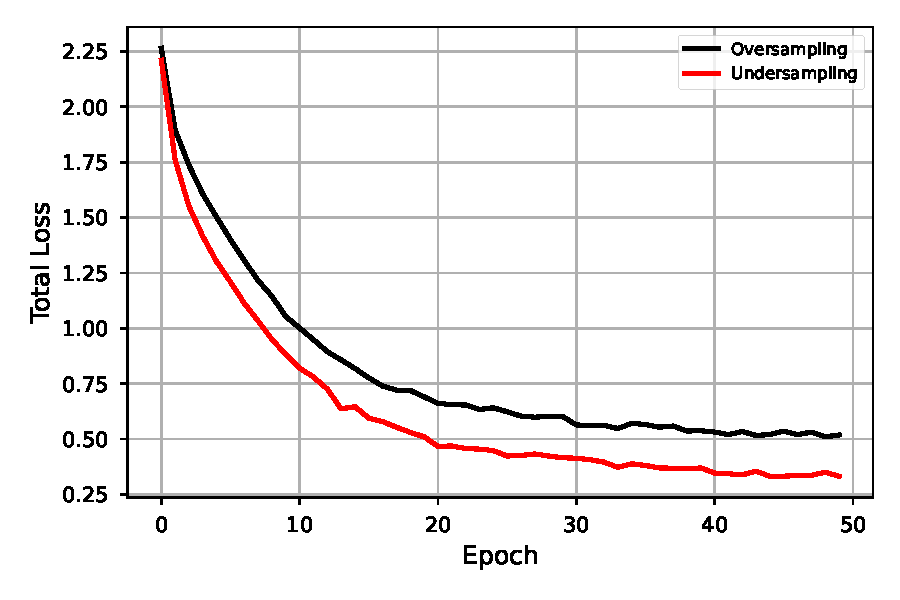
\includegraphics[width=0.6\textwidth]{loss_comparison.pdf}
    \caption{Training loss of vanilla oversampling and undersampling models.}
    \label{fig:1}
    \end{figure}

    \begin{figure}[h!]
    \centering
    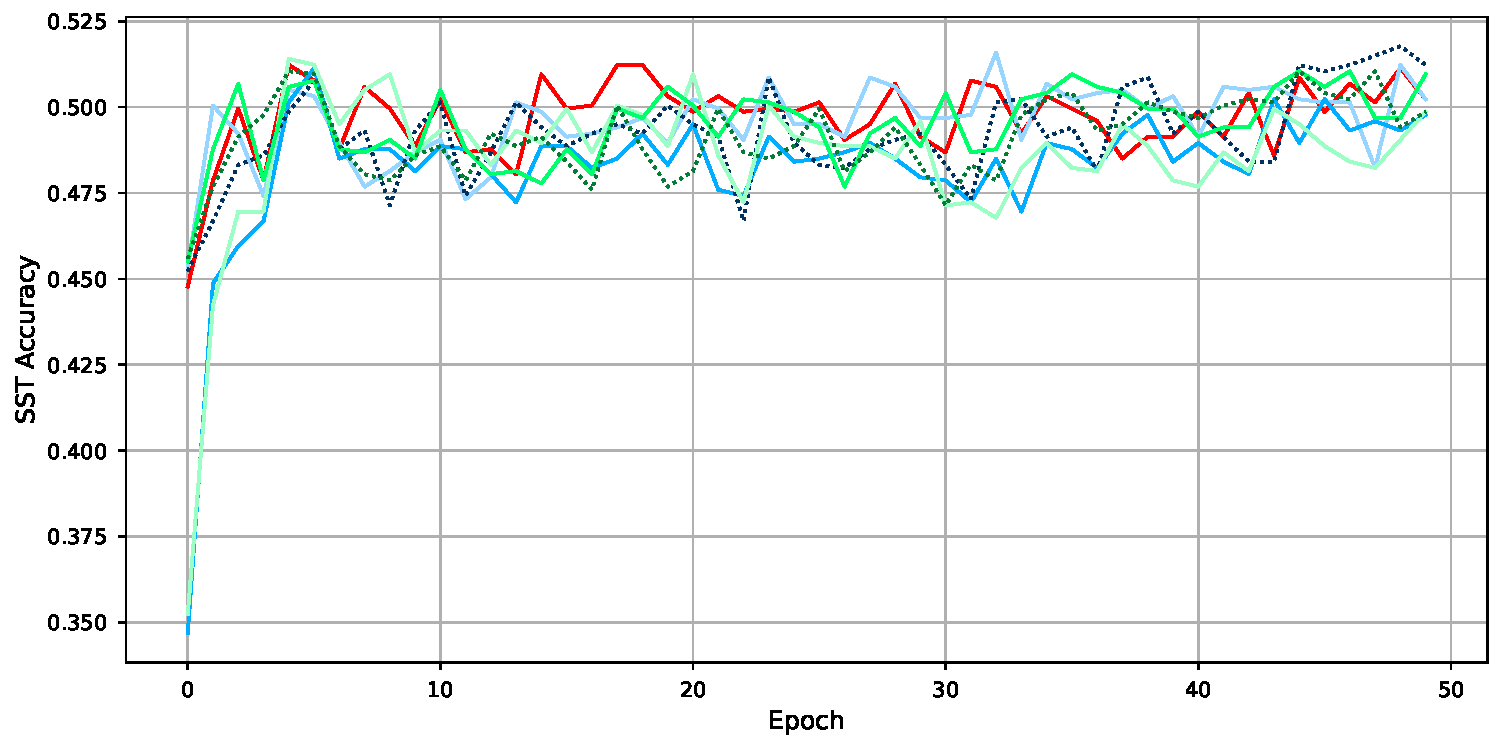
\includegraphics[width=0.8\textwidth]{accuracy_dev_sentiment.pdf}
    \end{figure}

    \begin{figure}[h!]
    \centering
    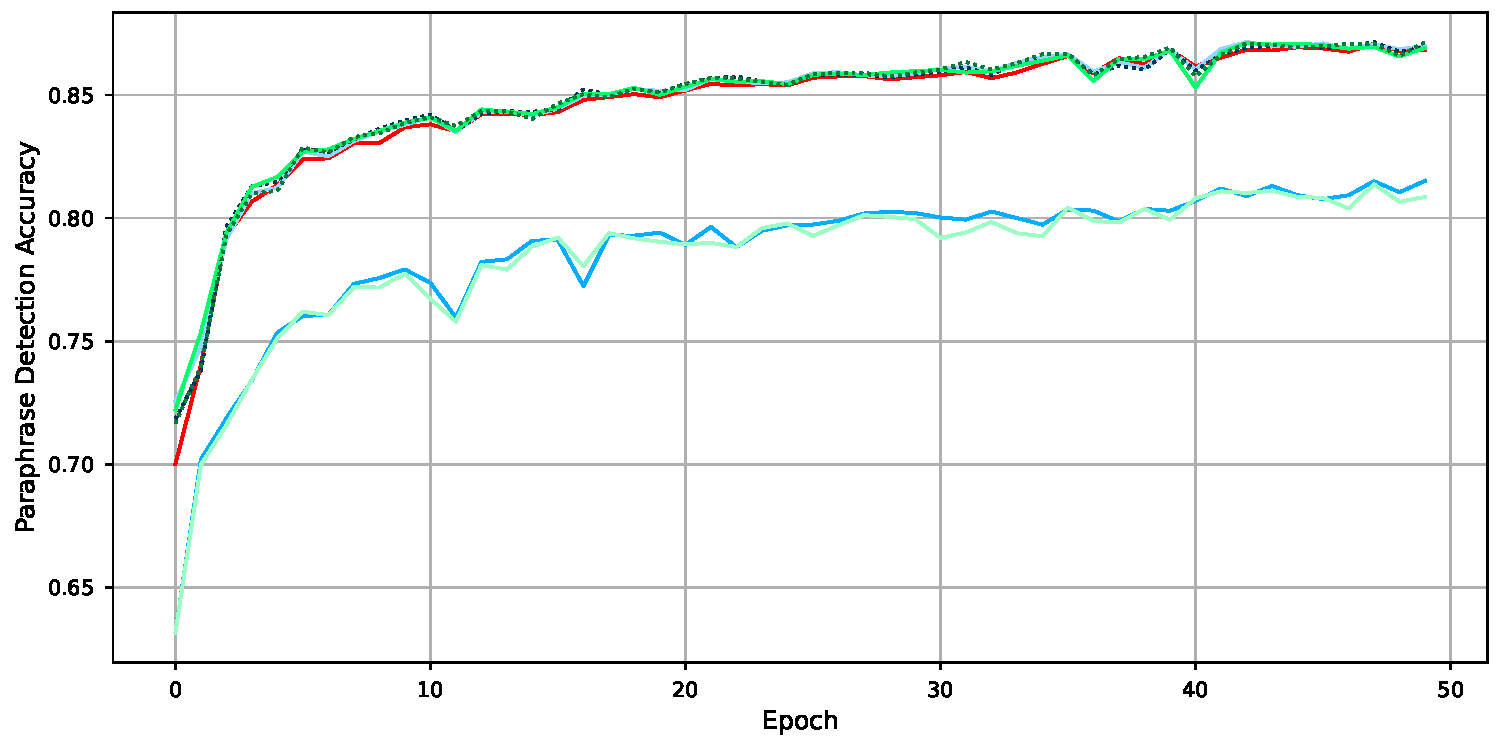
\includegraphics[width=0.8\textwidth]{accuracy_dev_paraphrase.pdf}
    \end{figure}

    \begin{figure}[h!]
    \centering
    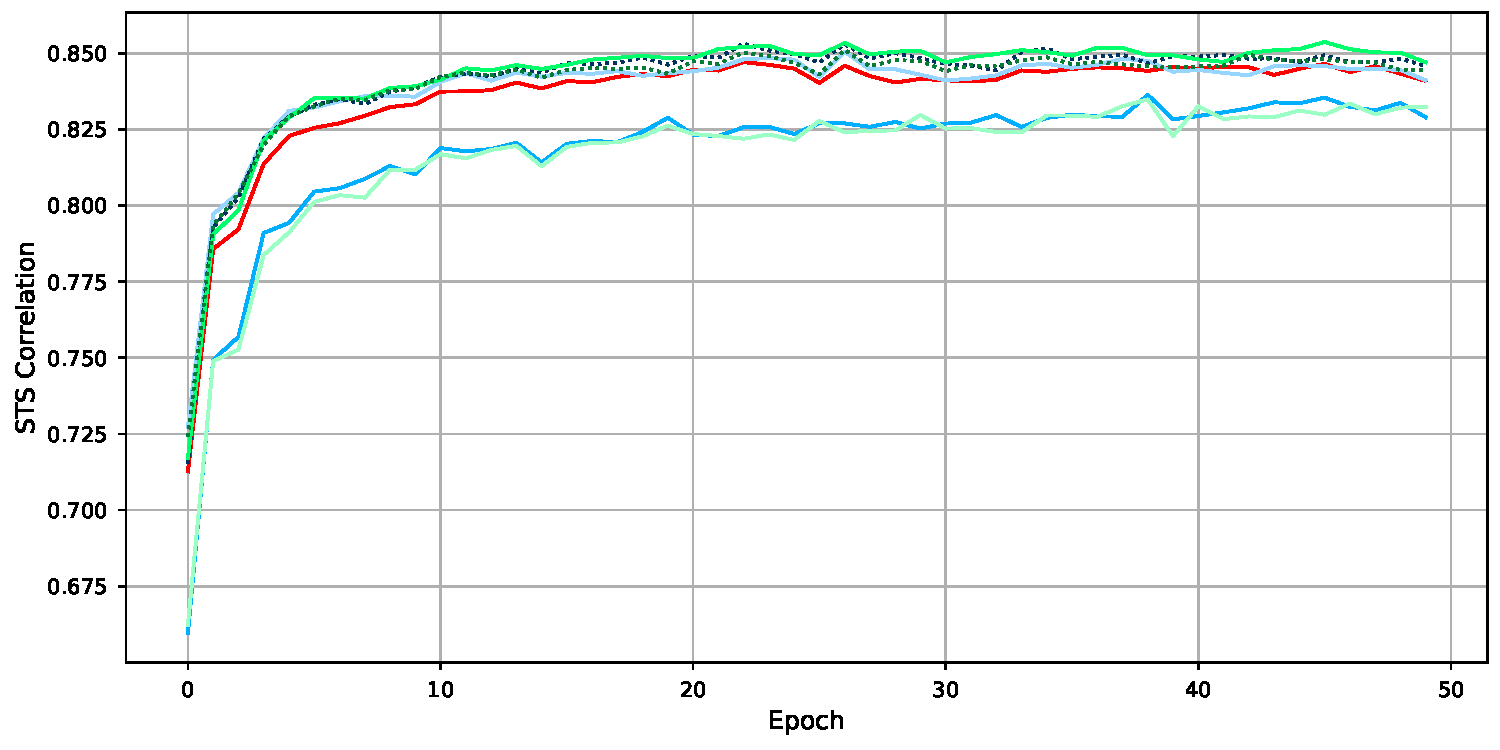
\includegraphics[width=0.8\textwidth]{correlation_dev_sts.pdf}
    \end{figure}

    \begin{figure}[h!]
    \centering
    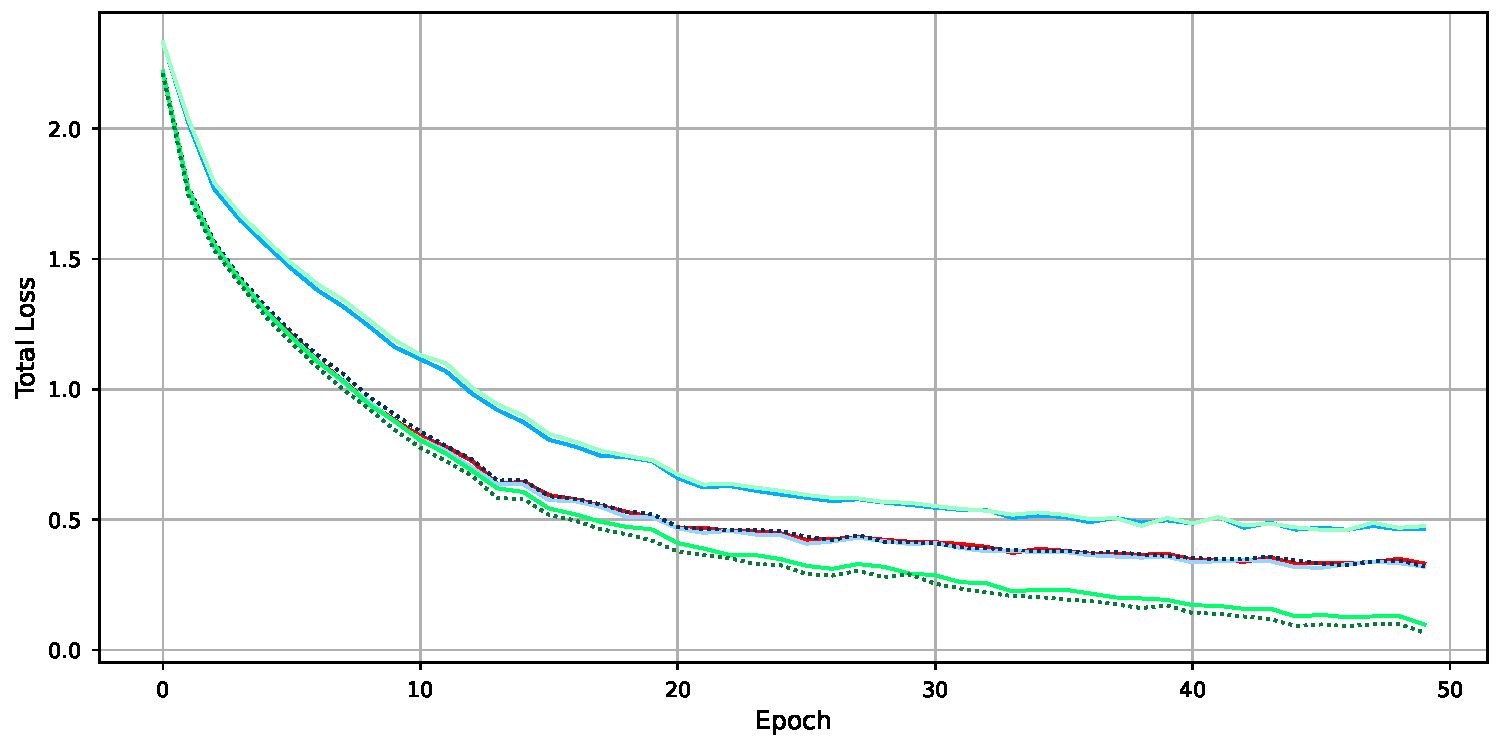
\includegraphics[width=0.8\textwidth]{loss_train_epoch.pdf}
    \end{figure}

    \begin{figure}[h!]
    \centering
    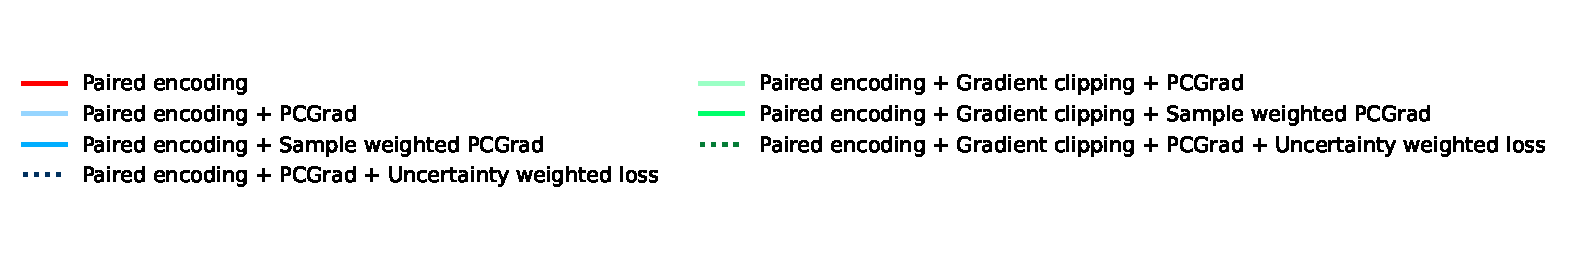
\includegraphics[width=\textwidth]{legend.pdf}
    \caption{SST accuracy, paraphrase accuracy, STS correlation, and total loss on the development set across 50 epochs. Note that the data of the weighted loss models are not to be directly compared to other data.}
    \label{fig:2}
    \end{figure}
    
    \newpage

  \subsection{Results}
  The table below shows the scores of models in the later experiments.
  \begin{table}[ht]
    \centering
    %\caption{}
    \label{tab:results}
    \begin{tabular}{l|cccc}
      \toprule
      Model & SST Acc & Para Acc & STS Corr & Dev Score\\
      \midrule
      Baseline & 0.490 & 0.748 & 0.478 & 0.659\\
      Cosine similarity for STS & 0.498 & 0.747 & 0.519 & 0.668\\
      CosineEmbeddingLoss for STS & 0.500 & 0.745 & 0.395 & 0.648\\
      Paired encoding & 0.501 & 0.871 & 0.846 & 0.765\\
      \makecell[l]{Paired encoding \\+ PCGrad} & 0.505 & \textbf{0.872} & 0.843 & 0.766\\
      \makecell[l]{Paired encoding \\+ Sample weighted PCGrad} & 0.498 & 0.815 & 0.829 & 0.742\\
      \makecell[l]{Paired encoding \\+ PCGrad + Uncertainty weighted loss} & 0.499 & \textbf{0.872} & 0.844 & 0.764 \\
      \makecell[l]{Paired encoding + Gradient clipping \\+ PCGrad} & \textbf{0.515} & 0.871 & 0.847 & \textbf{0.770}\\
      \makecell[l]{Paired encoding + Gradient clipping \\+ Sample weighted PCGrad} & 0.482 & 0.814 & 0.830 & 0.737\\
      \makecell[l]{Paired encoding + Gradient clipping \\+ PCGrad + Uncertainty weighted loss} & 0.494 & 0.871 & \textbf{0.850} & 0.763\\
      \bottomrule
    \end{tabular}
  \end{table}
  While the model with paired encoding, gradient clipping and PCGrad scores highest on overall score and SST Accuracy,
  the model with paired encoding and PCGrad has the highest Paragraph Detection Accuracy, and the last model has the highest STS Correlation.

\section{Analysis}
  \paragraph{Findings}
    \begin{itemize}
      \item \textbf{Models trained with oversampling perform worse than those trained with undersampling.}
      This reveals the negative statistical effect of a much larger dataset, which can be mitigated through random sampling.
      \item \textbf{Paired encoding outperforms cosine similarity and CosineEmbeddingLoss.}
      It demonstrates the strength of the self-attention mechanism, which is significantly better at capturing the similarities between sentences than simply comparing the embeddings geometrically.
      \item \textbf{Gradient techniques including PCGrad have positive but limited effects.}
      It might be the case that the three sentence-level tasks are similar and have limited conflicts in updates.
      The minimal impact of gradient clipping and uncertainty weighted loss suggests that the gradient updates from different datasets are neither excessively large nor highly uncertain.
      \item \textbf{No single best model excels at all three tasks simultaneously.}
      This indicates that among the techniques explored in our experiments, no definitive solution emerges.
      Alternative approaches not investigated in this work might hold the key to addressing these challenges.
    \end{itemize}

  \paragraph{Limitations}
    \begin{itemize}
    \item This project implemented only a limited set of multitask training techniques,
    leaving numerous potential solutions unexplored.
    \item The hyperparameters are never tuned in this project.
    Tuning learning rates and assigning specific weights to the tasks may further help the model to converge on sentiment analysis.
    \end{itemize}

\bibliographystyle{unsrt}
\bibliography{references}

\end{document}
